\subsection{Architekturentscheide}
Wesentliche Entscheide, welche wir während dem Projekt getroffen haben, sind hier detailliert begründet. Auch Gedanken oder Ideen, welche wir während der Analysephase hatten, dann aber wieder verworfen haben, sind hier mit Begründung aufgeschrieben.

\subsubsection{Domain-Design-Entscheid}
Schon sehr früh im Projekt kam die Idee auf, die BrainstormingFindings in verschiedene Arten zu unterteilen. Die Rede war von ``Software Architektur Lösung`` (SoftwareFinding) und ``Generelle Lösung`` (GeneralFinding). Siehe dazu Kapitel \ref{sec:sol-strategy}. Damit wollten wir erreichen, dass nicht jeder Ideentyp für jedes BrainstormingFinding zur Verfügung steht, zumal es auch nicht unbedingt für jede Kombination Sinn ergibt, diesen Ideentypen dafür zu verwenden. Zum Beispiel ist es wenig sinnvoll die PatternIdea bei einem GeneralFinding zu nutzen. Dies würde eher bei einem SoftwareFinding zum Einsatz kommen.

\begin{figure}[h]
	\centering
	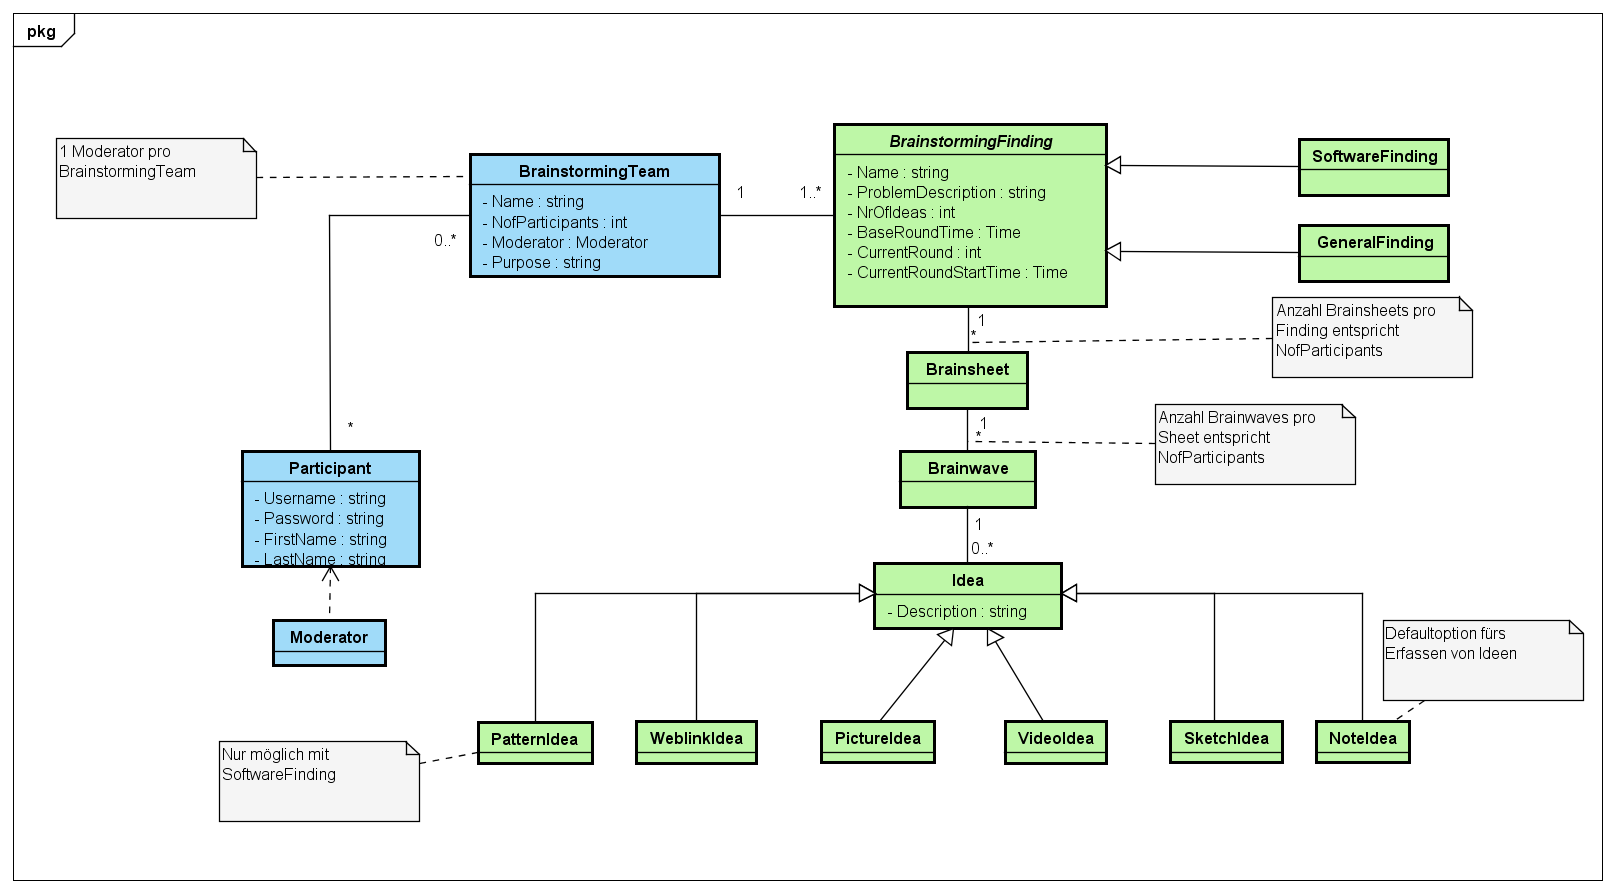
\includegraphics[width=1\linewidth]{img/domain-analyse/DomainModell-Methode635-Entwurf}
	\caption{Erster Entwurf vom Domain Modell BrainingOutOfBox}
	\label{fig:domainmodell-methode635-entwurf}
\end{figure}

Doch dabei kommt das Bedenken auf, was wenn es noch andere Patterns als nur Software-Patterns gibt, welche man zur Verfügung stellen will. Dann müssten noch mehr solcher logischen Zusammenhänge beachtet werden, was die Erweiterbarkeit der Applikation mit zunehmenden BrainstormingFinding Arten erschwert.

Je länger wir untereinander aber auch mit unserem Betreuer, Herr Zimmermann oder Silvan Gehrig darüber diskutierten, desto mehr kamen wir wieder auf unser ursprüngliches Domain-Design zurück, bei welchem es nur ein BrainstormingFinding gibt. 

Dabei ist die Idee, alle Ideentypen zwar anzubieten aber die Auswahl des passenden Ideentypen komplett dem Endnutzer zu überlassen. Dies birgt allerdings die Gefahr, die Benutzung der Applikation durch eine zu grosse Auswahl an Ideentypen zu verschlechtern. Dieses Problem kann aber durch eine durchdachte Aufteilung in der Benutzeroberfläche eingedämmt werden. Unserer Meinung nach ist mit dem verwendeten Domainmodell (siehe Abbildung \ref{fig:domainmodell-methode635}) die Erweiterbarkeit für zukünftige Arbeiten eher gegeben, da weniger Stellen im Code bearbeitet werden müssen. 

Aus diesem Grund haben wir uns für das ursprüngliche Domainmodell mit nur einem BrainstormingFinding entschieden. Die Tipps von arc42 bzw. der Solution Strategy konnten dennoch gemäss Tabelle \ref{tab:arc42-mapping} integriert werden.

\subsubsection{Architekturentscheide der Studienarbeit}
Nachfolgend listen wir die Entscheide auf, welche in der vorangegangenen Studienarbeit in Bezug auf die eingesetzten Technologien getroffen wurden. Es soll dem Leser nochmals  verständlich machen, warum genau diese Technologien für diese Arbeit gewählt wurden.
Die folgenden Kapitel sind daher der Studienarbeit \cite{methode635-sa} wortgetreu entnommen.

\paragraph*{Xamarin.Forms oder Xamarin native}\label{subsubsec:forms-vs-native}~\\
Für diesen Entscheid galt es zu evaluieren, welche User Controls für unsere Applikation die exotischsten sind. Dies, weil Xamarin.Forms eine Menge an Standard-Controls anbietet, die vom Framework selber in das jeweilige Betriebssystem konvertiert werden. Sind alle vorgesehenen Benutzerelemente in Forms enthalten, sparen wir uns die Zeit, betriebssystemspezifische Elemente zu entwickeln. 

Für unser Projekt haben wir folgende Benutzerelemente als exotisch oder kritisch definiert:
\begin{itemize}
	\item Canvas Control für Zeichnen einer Idee
	\item Camera Funktion für das Erkennen von Quick Response-Codes (QR-Codes)
	\item Verarbeitung und Generierung von QR-Codes
\end{itemize}

Nach einer Recherche stellte sich heraus, dass sich ein Canvas View von Google namens SkiaSharp eignet. Darauf lässt sich gemäss der Dokumentation zeichnen sowie definierte Formen einfügen. Dies könnte auch für eine Erweiterung spannend sein, in der Patterns in UML als Vorlage angeboten werden können.

Für die Kamera-Funktionalität steht ein NuGet-Packet (Xam.Media.Plugin) bereit, das uns diese Arbeit abnehmen wird.

Das Generieren und Lesen der QR-Codes ist an sich kein Problem von Xamarin.Forms, denn grundsätzlich müssen die von der Kamera generierten Files eingelesen und ins entsprechende QR-Code-Tool eingefügt werden. Hierfür eignet sich das NuGet ZXing.Net. 

Es stellte sich relativ rasch heraus, dass die gewünschten Funktionalitäten in Xamarin.Forms in ausreichender Qualität enthalten sind und uns das individuelle Entwickeln dadurch abgenommen wird.\\
\\


\paragraph*{Backend-Technologie}~\\

Neben den Vorteilen, wie der schlanken und zustandslosen Architektur des Play\-Frameworks, dem asynchronen und nicht-blockierenden Verhalten und den vielen unterstützten Bibliotheken, haben wir uns hauptsächlich dafür entschieden, weil wir in anderen Projekten schon sehr gute Erfahrungen mit dem PlayFramework gemacht haben.

Ein weiterer Grund bestand darin, dass das PlayFramework nicht nur in Scala sondern auch in Java geschrieben ist. Mit Java kennen wir uns beide gut aus und mussten uns so keine neue Programmiersprache aneignen.

Da wir uns schon relativ früh für eine MongoDB als Datenbanksystem entschieden hatten, fiel die Wahl erst recht auf das PlayFramework, als wir einen asynchronen MongoDB-Treiber für Java gefunden hatten.

\paragraph*{MongoDB als Datenbanksystem}~\\

MongoDB (abgeleitet von humongous) ist eine dokumentorientierte, einfache, dynamische und skalierbare NoSQL Datenbank, welche von der MongoDB Inc. entwickelt wird. 

Die Basis für das Speichern von Informationen bilden die sogenannten Documents. Die Datenobjekte werden in separaten Documents innerhalb einer Collection (anders als bei traditionellen relationalen Datenbanken in Spalten und Zeilen) gespeichert. Mit den Documents können zudem  hierarchische Strukturen und Relationen sehr einfach gespeichert werden.

Der Vorteil einer MongoDB Datenbank liegt darin, dass zusammengehörige Informationen gemeinsam in einem Document gespeichert werden. Dies ermöglicht einen schnellen Zugriff auf die Daten mittels der MongoDB Query Language. Da MongoDB zudem ohne Schemas auskommt, ist es nicht nötig, die Datenbank offline zu nehmen, wenn man ein neues Feld einfügen möchte.

Weitere Vorteile sind laut \href{DZone.com}{DZone.com} die hohe Performance, Verfügbarkeit (durch Replikas) und Skalierung (durch Sharding). Da alle Informationen zusammen in einem Document gespeichert sind, sind auch keine Joins zu anderen Tabellen notwendig. Auch unterstützt MongoDB Funktionen für die Speicherung von Geoinformationen.

Der Hauptgrund warum wir uns für MongoDB als Datenbanksystem entschieden haben, war die Tatsache, dass alle zusammengehörigen Informationen in einem Document abgelegt werden können. Auch die Möglichkeit hierarchische Strukturen (bei uns die \textit{Brainsheets}, \textit{Brainwaves} und \textit{Ideas}) einfach zu Speichern, hat uns viel Zeit erspart.

Die Mächtigkeit von relationalen Datenbanken im Bereich einer Auswertung, ist in unserem Projekt nicht notwendig. Daher haben wir auch von Beginn an auf das Paradigma der dokumentorientieren Datenbanken gesetzt. Grund warum wir uns schlussendlich für MongoDB und nicht für eine andere dokumentorientierte Datenbank entschieden haben ist, dass MongoDB Thema während dem Studium ist und wir schon einige Erfahrung damit hatten.
\\
\\

\paragraph*{Runden-Ende-Entscheid}~\\

Der Entscheid, wie eine Runde zu enden hat bzw. was passiert, wenn die Zeit in der laufenden Runde abläuft, der Participant aber noch nicht alle seine Ideen in die Brainwave gespeichert hat, hatten wir schon relativ früh in der Studienarbeit entschieden aber nirgends dokumentiert. Dies soll hier nachgeholt und begründet werden.

Grundsätzlich haben wir uns in solch einem Fall dazu entschlossen, lediglich jene Ideen in der Datenbank zu persistieren, welche auch in der Brainwave gespeichert sind. Im Umkehrschluss bedeutet das, dass alle Ideen, welche zu diesem Zeitpunkt nicht in der Brainwave gespeichert sind (betrifft nur die letzte erfasste Idee), verloren gehen. 

Der Grund warum wir uns dafür entschieden haben liegt einerseits darin, dass dies die einfachste Lösung für die geschilderte Situation darstellt. Da dies zudem nur eine Idee betreffen kann, kann auch nur maximal diese Idee 'verloren' gehen. 

Zudem wird bei der originalen Version mit Papier gleich verfahren. Auch dort wird unabhängig, ob ein Participant alle Ideen ausfüllen konnte oder nicht, das Blatt weitergereicht. 